% The log embedding of the units of the real cubic field Q(2cos(2pi/7)), projected to the plane x1+x2+x3=0 (generated).
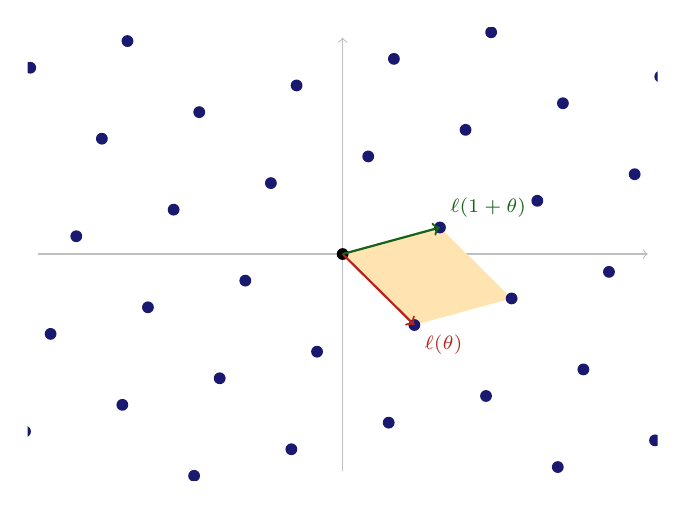
\begin{tikzpicture}[scale=1.25]
\clip (-3.2,-2.3) rectangle (3.2,2.3);
\draw[black!25,->] (-3.1,0)--(3.1,0); \draw[black!25,->] (0,-2.2)--(0,2.2);
\fill[Orange!30] (0,0)--(0.729,-0.721)--(1.717,-0.451)--(0.989,0.270)--cycle;
\fill[MidnightBlue] (-3.174,1.893) circle (0.06);
\fill[MidnightBlue] (-2.186,2.164) circle (0.06);
\fill[MidnightBlue] (-2.446,1.172) circle (0.06);
\fill[MidnightBlue] (-1.457,1.442) circle (0.06);
\fill[MidnightBlue] (-0.468,1.713) circle (0.06);
\fill[MidnightBlue] (0.521,1.983) circle (0.06);
\fill[MidnightBlue] (1.509,2.253) circle (0.06);
\fill[MidnightBlue] (-2.706,0.181) circle (0.06);
\fill[MidnightBlue] (-1.717,0.451) circle (0.06);
\fill[MidnightBlue] (-0.729,0.721) circle (0.06);
\fill[MidnightBlue] (0.260,0.992) circle (0.06);
\fill[MidnightBlue] (1.249,1.262) circle (0.06);
\fill[MidnightBlue] (2.238,1.532) circle (0.06);
\fill[MidnightBlue] (3.227,1.803) circle (0.06);
\fill[MidnightBlue] (-2.967,-0.811) circle (0.06);
\fill[MidnightBlue] (-1.978,-0.541) circle (0.06);
\fill[MidnightBlue] (-0.989,-0.270) circle (0.06);
\fill[black] (0.000,0.000) circle (0.06);
\fill[MidnightBlue] (0.989,0.270) circle (0.06);
\fill[MidnightBlue] (1.978,0.541) circle (0.06);
\fill[MidnightBlue] (2.967,0.811) circle (0.06);
\fill[MidnightBlue] (-3.227,-1.803) circle (0.06);
\fill[MidnightBlue] (-2.238,-1.532) circle (0.06);
\fill[MidnightBlue] (-1.249,-1.262) circle (0.06);
\fill[MidnightBlue] (-0.260,-0.992) circle (0.06);
\fill[MidnightBlue] (0.729,-0.721) circle (0.06);
\fill[MidnightBlue] (1.717,-0.451) circle (0.06);
\fill[MidnightBlue] (2.706,-0.181) circle (0.06);
\fill[MidnightBlue] (-1.509,-2.253) circle (0.06);
\fill[MidnightBlue] (-0.521,-1.983) circle (0.06);
\fill[MidnightBlue] (0.468,-1.713) circle (0.06);
\fill[MidnightBlue] (1.457,-1.442) circle (0.06);
\fill[MidnightBlue] (2.446,-1.172) circle (0.06);
\fill[MidnightBlue] (2.186,-2.164) circle (0.06);
\fill[MidnightBlue] (3.174,-1.893) circle (0.06);
\draw[->,thick,BrickRed] (0,0)--(0.729,-0.721) node[below right,font=\scriptsize]{$\ell(\theta)$};
\draw[->,thick,ForestGreen!70!black] (0,0)--(0.989,0.270) node[above right,font=\scriptsize]{$\ell(1+\theta)$};
\end{tikzpicture}
